\chapter{Electrons in a Magnetic Field, Quantum Hall Effect and Landau Levels}

Last time we built the general machinery of topological band structure: the Kubo formula for the
Hall conductivity, its rewriting as an integral of Berry curvature, the Chern number as the
resulting topological invariant, and the bulk-boundary correspondence that ties a nonzero Chern
number to a protected chiral edge state. We worked all of that machinery through two concrete
examples, the SSH chain and a gapped Dirac cone on the honeycomb lattice (the Haldane
construction), and we did it quite deliberately without ever turning on a magnetic field. That
was a promissory note: session 2 had already told us that a Bloch Hamiltonian's dispersion comes
in three archetypes, parabolic, Dirac, and flat, and the flat-band case, the one that gives a
literal magnetic field its own dedicated topological story, was left for today. So let us pick up
exactly where we left off. Today we run session 3's Chern-number machinery through the flat-band
case in full: the integer quantum Hall effect, Landau levels as topological flat bands, and then,
once we let those flat bands become genuinely many-body objects, the Laughlin wavefunction,
fractional charge, and anyonic statistics, the simplest example of fractionalization we will meet
in this course. We will close by turning the telescope back around: the Haldane model gives us a
quantized Hall conductance with no magnetic field at all, and we will see explicitly that it and
the ordinary quantum Hall state are two faces of the very same topological phase.

\section{Where the quantum Hall state shows up}

The first thing worth appreciating about the quantum Hall state is that it is not the property of
one particular material; it is a state of matter that a whole family of two-dimensional electron
systems can realize, each with its own convenient energy and temperature scale.

\begin{itemize}
\item \textbf{Semiconductor quantum wells}, historically gallium arsenide (GaAs), were the original
  platform. There the electrons are essentially parabolic (ordinary, quadratic-dispersion)
  electrons, the relevant energy scale grows linearly in the magnetic field, and the numbers work
  out to roughly one millielectronvolt for laboratory-accessible fields, which is why GaAs quantum
  Hall physics needs temperatures on the order of one kelvin.
\item \textbf{Two-dimensional materials}, and graphene above all, realize the same physics but with Dirac
  electrons rather than parabolic ones. As we will derive explicitly below, that changes the
  energy scale to grow as the square root of the field rather than linearly, and the slides give
  the concrete numbers: roughly two orders of magnitude larger, around 100 millielectronvolts, high
  enough that graphene's quantum Hall plateaus survive up to about 100 K, and in the best samples
  essentially up to room temperature.
\end{itemize}

Whatever the platform, the common thread is the one we already met last session: an observable,
the Hall conductance, comes out exactly quantized, and that quantization is a statement about
topology rather than about any particular material's chemistry.

\section{Measuring the Hall conductance}

The experiment itself is simple to state. Take a two-dimensional system, apply a voltage along
one in-plane direction (call it $y$), and measure the resulting current along the perpendicular
in-plane direction ($x$). The ratio of that transverse current to the applied voltage is the Hall
conductance, and it is this object that gets quantized in the quantum Hall regime.

A real device realizing this measurement is a two-dimensional electron gas (2DEG) contacted by
several finger gates: a voltage is imposed between a top and a bottom gate, and the current is
read off between two gates arranged along $x$, with everything wired through metallic leads.
The device geometry itself carries no new physics beyond what we need conceptually, so we will not
dwell on it further; the slide deck's device figures are worth a glance for the real-world picture,
but the notes from here on work with the idealized two-dimensional system.

\section{From the Kubo formula to the Chern number, briefly}

We derived this result in full last session, so let us not repeat fifteen lines of algebra that
would look almost identical; instead let us recall the logic and confirm that it applies unchanged
here. Second-order perturbation theory (the Kubo formula) gives the transverse conductivity as a
sum, over all pairs of occupied and empty bands, of matrix elements of $\partial H/\partial k_x$
and $\partial H/\partial k_y$ divided by energy differences. Using the identity that relates
$\partial H/\partial k$ to the derivative of the eigenstates themselves (differentiate the
eigenvalue equation $H(\mathbf{k})|u_\mathbf{k}\rangle = \varepsilon(\mathbf{k})|u_\mathbf{k}\rangle$
with respect to $\mathbf{k}$), every explicit energy denominator cancels, and what survives depends
only on the wavefunctions: the Berry connection $\mathbf{A}(\mathbf{k}) = i\langle
u_\mathbf{k}|\nabla_\mathbf{k}|u_\mathbf{k}\rangle$ and its curl, the Berry curvature
$\Omega(\mathbf{k}) = \nabla_\mathbf{k}\times\mathbf{A}(\mathbf{k})$. Summing over occupied bands
and integrating over the Brillouin zone (a closed, compact manifold, a torus) gives an integer,

\begin{equation}
\sigma_{xy} = \frac{e^2}{h}\, C, \qquad C = \frac{1}{2\pi}\sum_{n\,\text{occ.}}\int_{\text{BZ}} \Omega_n(\mathbf{k})\, d^2k \in \mathbb{Z},
\end{equation}

the Chern number of the occupied bands. This is the same statement as session 3's: the Hall
conductance is not just quantized, it is a topological invariant, insensitive to any smooth
deformation of the Hamiltonian that does not close the bulk gap. What is new today is not this
derivation; it is the specific band structure we are going to plug into it, a magnetic field's
Landau levels, and everything that follows once we ask what the many-body ground state of a
\emph{partially filled} Landau level looks like.

\section{Landau levels as Chern-number-one flat bands}

A two-dimensional electron gas in a perpendicular magnetic field develops a set of completely flat
bands, the Landau levels, indexed $n=0,1,2,\dots$. ``Flat'' here means dispersionless: the energy
does not depend on momentum at all (we will derive exactly why in Section 4.9). Despite carrying
no dispersion, each Landau level carries a finite, and in fact minimal nonzero, Chern number:
$C=1$. If the chemical potential sits between the $N$-th and $(N+1)$-th Landau level, the total
Chern number of the occupied bands is simply the sum of $N$ individual contributions of $1$,

\begin{equation}
C_{\text{tot}} = \sum_{n=1}^{N} C_n = N \quad\Longrightarrow\quad \sigma_{xy} = N\,\frac{e^2}{h},
\end{equation}

an integer directly counting the number of filled Landau levels. This is the integer quantum Hall
effect: a state built entirely from flat, dispersionless bands, whose Hall conductance is
nonetheless an exact, sharply quantized integer multiple of $e^2/h$.

\section{Why an insulating bulk still conducts: edge states}

Here is the obvious puzzle. If the chemical potential sits in a gap between two Landau levels, the
bulk of the sample is, by definition, an insulator: no partially filled band, no bulk states at
the Fermi energy. So how can such a system carry a finite, quantized current at all?

The answer, exactly as in session 3's general bulk-boundary argument, is that a nonzero Chern
number cannot simply end: at any interface where the Chern number changes (here, the boundary
between a Chern-$N$ sample and the vacuum, which has $C=0$), there must be $N$ protected, gapless,
chiral edge modes. A chiral mode propagates in only one direction; the number of edge modes at an
interface equals the difference in Chern number across it. Every real sample is finite, so it
always has an edge, and the edge states are always there, whether or not we are thinking about
them. Applying a voltage between the top and bottom edges of the sample simply creates an
imbalance between right-moving and left-moving edge electrons, and that imbalance is exactly the
quantized Hall current.

The band structure of a ribbon (a sample infinite in $y$, finite in $x$) makes the picture
completely explicit: alongside the flat, dispersionless bulk Landau levels, one finds a set of
dispersive states localized at the left edge, all propagating in one direction, and a mirror set
localized at the right edge, propagating in the opposite direction. Because a given propagation
direction is tied to a \emph{location} (left edge or right edge), an impurity sitting on the left edge
simply cannot scatter a left-moving electron into a right-moving one: the right edge is macroscopically
far away. There is no available final state, so there is no backscattering, and the edge transport
is dissipationless. Figure~\ref{fig:s04:ribbon} puts the ribbon spectrum and its real-space
counterpart side by side, and shows the chiral modes crossing the chemical potential.

% Session 4 -- the ribbon spectrum: flat bulk Landau levels plus chiral edge
% branches, and why an impurity cannot backscatter an edge electron.
% Placement: sec. "Why an insulating bulk still conducts: edge states", after the
% ribbon / no-backscattering paragraph.
% Rendered by figures/blender/s04f01_ribbon.py, labels in figures/overlays/s04f01_ribbon.tex.
\begin{aqmfigure}{fig:s04:ribbon}{The quantum Hall ribbon. (a) The spectrum of a strip that is
infinite along $y$ and finite along $x$, computed for a width of $12\,\ell_B$ with hard walls. In
the bulk the Landau levels (4.6) are exactly flat, so they carry no current at all, but near each
boundary the guiding centre $x_0=\hbar k_y/B$ is pushed into the wall and the level bends up
strongly. These bending branches are the edge states, and each of them crosses the chemical
potential, the translucent plane, exactly once per edge, at the balls, so the number of chiral modes
at a given edge is equal to the number $N$ of filled Landau levels, here $N=2$. (b) The same
statement in real space, seen from above. The branches with $k_y>0$ have
$v_y=\hbar^{-1}\partial_{k_y}E>0$ and live on the right edge, and the branches with $k_y<0$ move in
the opposite direction and live on the left edge. To reverse the velocity of an electron we would
therefore have to move it to the other side of the sample, which no local impurity can do, and this
is why the edge transport has no dissipation.}
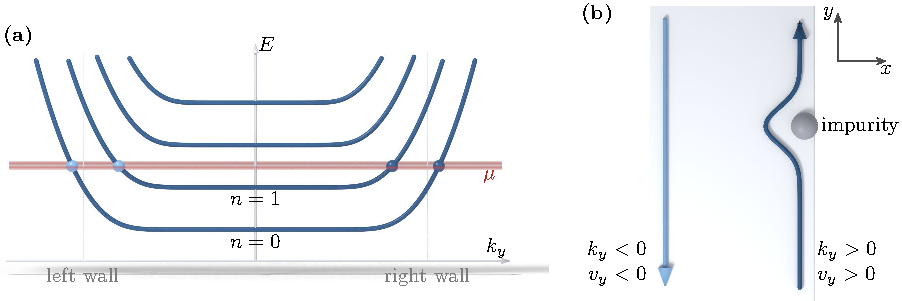
\includegraphics{figures/pdf/s04f01_ribbon.pdf}
\end{aqmfigure}


\begin{notebookbox}{\texttt{session4.ipynb}, ``Localization of the edge states in the quantum Hall effect in a ribbon'' (Challenge), and ``Localization of the edge states in the quantum Hall effect in an island'' (Challenge)}
Build a finite ribbon and a finite island in a magnetic field and look directly at where the
edge-state wavefunctions live in real space, confirming the left/right (or perimeter) separation
that the no-backscattering argument above depends on.
\end{notebookbox}

\section{The experimental signature: quantized Hall plateaus}

Sweeping the magnetic field on a real 2DEG shows this transition directly. At low field, before
the quantum regime sets in, the Hall resistance grows linearly with $B$, exactly the classical
Hall effect from ordinary electromagnetism. Once the field reaches the tesla range (the precise
scale depends on the material, tracking the Landau-level spacing derived below), a staircase of
sharp plateaus appears in the Hall resistance instead. As the field increases further, the
cyclotron energy $\hbar\omega_c$ grows, so fewer and fewer Landau levels remain below a fixed
chemical potential; each time the chemical potential sweeps past a Landau level, the number of
filled levels $N$ in (4.2) drops by one, and the Hall resistance jumps to the next quantized
plateau.

\section{Coupling electrons to a magnetic field: minimal coupling and the Peierls substitution}

To go beyond this phenomenology and actually derive the Landau level spectrum, we need to know how
to put a magnetic field into a Hamiltonian at all. Classically, a magnetic field $\mathbf{B} =
\nabla\times\mathbf{A}$ enters the equations of motion through the canonical momentum,

\begin{equation}
\boldsymbol{\pi} = \mathbf{p} - e\mathbf{A},
\end{equation}

replacing the ordinary momentum $\mathbf{p}$ everywhere it appears; computing the resulting
equations of motion reproduces the familiar Lorentz force law. Throughout this session we set the
electron charge magnitude and the speed of light to one (as the slides implicitly do), keeping only
$\hbar$ explicit where the Landau level spacing needs it. The same replacement (4.3) works
unchanged in quantum mechanics, with $\mathbf{p}\to-i\hbar\nabla$: minimal coupling turns the free
Hamiltonian $p^2/2m$ into $\pi^2/2m$, and similarly for the Dirac Hamiltonian below.

One subtlety is unavoidable: $\mathbf{A}$ is never unique. Any $\mathbf{A}\to\mathbf{A}+\nabla\chi$
for a scalar function $\chi$ gives the same physical field $\mathbf{B}$, so we always have to pick
a gauge. There are two gauges we will actually need, the Landau gauge and the symmetric gauge, and
we will meet both in Section 4.8. A related, and slightly counterintuitive, point: applying a
uniform out-of-plane field does not itself break the in-plane translational symmetry of the
physical system, but \emph{every} choice of $\mathbf{A}$ realizing that field breaks translational
symmetry formally, in one direction or in both. Which symmetry survives, and how much of it, is a
gauge choice, not a physical one.

The minimal-coupling replacement (4.3) is the natural route for continuum models: Schrödinger or
Dirac electrons, where we directly write down and solve a differential equation. For a
tight-binding model, written in real-space orbitals, the more natural route puts the field's
dependence into the wavefunctions rather than the Hamiltonian, via a local gauge transformation.
Concretely, the hopping amplitude $t_{ij}$ is, by definition, an overlap between the orbital
wavefunctions at sites $i$ and $j$; folding the vector potential into those wavefunctions
renormalizes every hopping by a complex phase equal to the line integral of $\mathbf{A}$ between
the two sites,

\begin{equation}
t_{ij} \;\longrightarrow\; t_{ij}\, \exp\!\left(i\int_{\mathbf{R}_i}^{\mathbf{R}_j} \mathbf{A}\cdot d\boldsymbol{\ell}\right),
\end{equation}

the \textbf{Peierls substitution}. It is the tight-binding counterpart of minimal coupling, and the two
give the same physics: at low energies, expanding a Peierls-substituted tight-binding model
reproduces the continuum minimal-coupling Hamiltonian directly.

\section{Choosing a gauge: Landau versus symmetric}

For a uniform field $\mathbf{B} = B\hat{z}$, two gauges will matter to us.

\begin{itemize}
\item The \textbf{Landau gauge}, $\mathbf{A} = (0, Bx, 0)$, puts all the spatial dependence into a single
  coordinate, $x$. Since $\mathbf{A}$ has no $y$-dependence, the Hamiltonian built from it still
  commutes with $p_y$ (translations along $y$ remain a good symmetry), but not with $p_x$. This
  gauge preserves \emph{one} translational symmetry, which is exactly what we need to talk about a band
  structure at all, and it is the gauge behind every ribbon calculation in this session.
\item The \textbf{symmetric gauge}, $\mathbf{A} = \tfrac{B}{2}(-y, x, 0)$, breaks both translational
  symmetries but preserves the system's rotational symmetry instead. It is the natural gauge for
  writing down many-body wavefunctions with good angular momentum, which is exactly what we need
  once we get to the fractional quantum Hall state in Section 4.13 onward.
\end{itemize}

Figure~\ref{fig:s04:gauge} makes the difference concrete by writing both gauges as Peierls phases
(4.4) on a square lattice: the individual bond phases look nothing alike, but the sum around any
plaquette --- the only gauge-invariant combination, and the only thing the electrons respond to
--- is the same flux in both.

% Session 4 -- Peierls phases on a square lattice in two different gauges, and the
% gauge-invariant plaquette sum.
% Placement: sec. "Choosing a gauge: Landau versus symmetric", after the two bullets.
%
% All phases are the line integrals of (4.4) in units where the lattice constant,
% e and hbar are one, so \varphi = B a^2 is the flux through one plaquette.
%   Landau  A = (0,Bx,0)      : horizontal bonds 0, vertical bond in column x is x\varphi.
%   Symmetric A = (B/2)(-y,x,0): vertical bond in column x is x\varphi/2,
%                                horizontal bond in row y is -y\varphi/2.
% Both give the same counterclockwise plaquette sum \varphi.
\begin{aqmfigure}{fig:s04:gauge}{Two gauges for the same magnetic field, written as Peierls phases
(4.4) on a square lattice. (a) In the Landau gauge the horizontal bonds carry no phase at all and
the vertical bond in column $x$ carries $x\varphi$: the phase pattern depends on $x$ but not on
$y$, so translations along $y$ are still an exact symmetry and a band structure in $k_y$ still
exists. (b) In the symmetric gauge every bond carries a phase and none of them matches (a), so no
translation survives, but the pattern is invariant under rotation about the plaquette centre.
Nothing physical distinguishes the two: going once around any plaquette, the individual phases add
up to the same $\varphi$, which is the flux through that plaquette. The bond phases are a gauge
choice, the loop sum is not, and it is the loop sum alone that the electrons respond to.}

\begin{tikzpicture}[x=1cm, y=1cm]

% =============================== helper macro ===============================
% \aqmlattice draws the 3x2 patch of sites and bonds at the current origin.
\newcommand{\aqmpatch}{%
  \foreach \i in {0,1,2} {
    \draw[aqmbond] (1.62*\i,0) -- (1.62*\i,1.62);
  }
  \foreach \j in {0,1} {
    \draw[aqmbond] (0,1.62*\j) -- (3.24,1.62*\j);
  }
  \foreach \i in {0,1,2} {
    \foreach \j in {0,1} {
      \node[aqmsite] at (1.62*\i,1.62*\j) {};
    }
  }
  % circulation arrows, one per plaquette
  \foreach \c in {0.81,2.43} {
    \draw[aqm, draw=aqmbroken, line width=\aqmthinwidth,
          -{Stealth[length=4pt,width=3.2pt]}]
      (\c+0.30,0.81) arc (0:305:0.30);
  }
}

% ============================ (a) Landau gauge ==============================
\begin{scope}[shift={(0,0)}]
  \aqmpatch
  % vertical bonds: phase x*varphi
  \node[aqmlabsmall, fill=white, inner sep=1.4pt] at (0,0.81)    {$0$};
  \node[aqmlabsmall, fill=white, inner sep=1.4pt] at (1.62,0.81) {$\varphi$};
  \node[aqmlabsmall, fill=white, inner sep=1.4pt] at (3.24,0.81) {$2\varphi$};
  % horizontal bonds: no phase
  \node[aqmlabsmall, fill=white, inner sep=1.4pt] at (0.81,0)    {$0$};
  \node[aqmlabsmall, fill=white, inner sep=1.4pt] at (2.43,0)    {$0$};
  \node[aqmlabsmall, fill=white, inner sep=1.4pt] at (0.81,1.62) {$0$};
  \node[aqmlabsmall, fill=white, inner sep=1.4pt] at (2.43,1.62) {$0$};

  \node[aqmpanel, anchor=south] at (1.62,2.30) {(a) Landau gauge};
  \node[aqmlabsmall, anchor=south] at (1.62,1.96) {$\mathbf{A}=(0,Bx,0)$};

  \foreach \i/\lb in {0/{$x{=}0$},1/{$1$},2/{$2$}} {
    \node[aqmlabmuted, anchor=north] at (1.62*\i,-0.30) {\lb};
  }
  \node[aqmlabsmall, anchor=north, align=center] at (1.62,-0.86)
    {no $y$-dependence: $[H,p_y]=0$,\\[-1pt]so a band structure in $k_y$ survives};
\end{scope}

% ========================== (b) symmetric gauge =============================
\begin{scope}[shift={(6.6,0)}]
  \aqmpatch
  % vertical bonds: phase x*varphi/2, columns x = -1,0,1
  \node[aqmlabsmall, fill=white, inner sep=1.4pt] at (0,0.81)    {$-\tfrac{\varphi}{2}$};
  \node[aqmlabsmall, fill=white, inner sep=1.4pt] at (1.62,0.81) {$0$};
  \node[aqmlabsmall, fill=white, inner sep=1.4pt] at (3.24,0.81) {$+\tfrac{\varphi}{2}$};
  % horizontal bonds: phase -y*varphi/2, rows y = -1/2, +1/2
  \node[aqmlabsmall, fill=white, inner sep=1.4pt] at (0.81,0)    {$+\tfrac{\varphi}{4}$};
  \node[aqmlabsmall, fill=white, inner sep=1.4pt] at (2.43,0)    {$+\tfrac{\varphi}{4}$};
  \node[aqmlabsmall, fill=white, inner sep=1.4pt] at (0.81,1.62) {$-\tfrac{\varphi}{4}$};
  \node[aqmlabsmall, fill=white, inner sep=1.4pt] at (2.43,1.62) {$-\tfrac{\varphi}{4}$};

  \node[aqmpanel, anchor=south] at (1.62,2.30) {(b) symmetric gauge};
  \node[aqmlabsmall, anchor=south] at (1.62,1.96)
    {$\mathbf{A}=\tfrac{B}{2}(-y,x,0)$};

  \foreach \i/\lb in {0/{$x{=}{-}1$},1/{$0$},2/{$+1$}} {
    \node[aqmlabmuted, anchor=north] at (1.62*\i,-0.30) {\lb};
  }
  \node[aqmlabsmall, anchor=north, align=center] at (1.62,-0.86)
    {depends on $x$ \emph{and} $y$: no translation\\[-1pt]survives, but the rotation does};
\end{scope}

% =========================== the shared punchline ===========================
\node[aqmboxbroken, anchor=north, align=center] at (4.86,-1.98)
  {going once counterclockwise around \emph{any} plaquette, both gauges give the same
   $\oint\mathbf{A}\cdot d\boldsymbol\ell=\varphi=\Phi_\square$\\[2pt]
   \textcolor{aqmmuted}{the bond phases are a gauge choice; the loop sum is the physical flux}\\[2pt]
   \textcolor{aqmmuted}{(each label is the phase for hopping in the $+x$ or $+y$ direction)}};

\end{tikzpicture}

\end{aqmfigure}


\section{Landau levels of Schrödinger electrons}

Let us now actually solve for the spectrum, starting with the simplest possible case: free
electrons, no lattice, no potential beyond the field itself, dispersion $p^2/2m$ before the field
is switched on. With minimal coupling and the Landau gauge $\mathbf{A}=(0,Bx,0)$,

\begin{equation}
H = \frac{\pi_x^2+\pi_y^2}{2m} = \frac{p_x^2}{2m} + \frac{(p_y-Bx)^2}{2m}.
\end{equation}

We take the carrier charge to be $+e$ in (4.3) and set $e=\hbar=1$ throughout. This is a
bookkeeping choice, but not a free one: it fixes $[\pi_x,\pi_y]=+i\hbar^2/\ell_B^2$, which is the
convention the ladder operators of Section 4.10 and the holomorphic wavefunctions of Section 4.13
are built on. For an electron, of charge $-e$, every cyclotron orbit and every edge current below
circulates the other way, and nothing else changes.

Because $\mathbf{A}$ has no $y$-dependence, $[H,p_y]=0$, so we can look for eigenstates of the form
$\psi(x,y) = e^{ik_y y}\phi(x)$. Replacing $p_y\to\hbar k_y$ turns (4.5) into a purely
one-dimensional problem in $x$,

\begin{equation*}
H\phi(x) = \left[\frac{p_x^2}{2m} + \frac{B^2}{2m}\Big(x-\frac{\hbar k_y}{B}\Big)^2\right]\phi(x),
\end{equation*}

which is exactly the Hamiltonian of a quantum harmonic oscillator, centered at $x_0 = \hbar
k_y/B$ (a shift absorbed by a change of variable, exactly as the lecture describes) with frequency
$\omega_c = B/m$, the cyclotron frequency. Solving it with the same ladder-operator machinery as
the ordinary harmonic oscillator gives

\begin{equation}
E_n = \hbar\omega_c\left(n+\frac{1}{2}\right), \qquad n=0,1,2,\dots,
\end{equation}

completely independent of $k_y$: every value of $k_y$ (equivalently, every choice of guiding center
$x_0$) gives the same energy, which is exactly why the Landau levels are flat bands, and why each
one carries a macroscopic degeneracy proportional to the sample area. Figure~\ref{fig:s04:guidingcenter}
draws that mechanism directly: the same well parked in different places, and the degeneracy
counted as one orbital per flux quantum through the sample. Plugging in real physical
constants for a GaAs-scale field gives the millielectronvolt scale quoted in Section 4.1.

% Session 4 -- why Landau levels are flat: the Landau-gauge reduction turns every
% k_y into the same harmonic oscillator, only displaced.
% Placement: sec. "Landau levels of Schroedinger electrons", after equation (4.6).
%
% LAYOUT NOTE: two pgfplots axes in one tikzpicture; the second is placed off the
% first with "at={($(ax1.south east)+(...)$)}". Everything inside each axis is in
% axis cs, nothing is drawn in bare tikzpicture coordinates.
\begin{aqmfigure}{fig:s04:guidingcenter}{Why the Landau levels are flat. (a) In the Landau gauge each
$k_y$ reduces (4.5) to a one-dimensional harmonic oscillator in $x$, identical in every respect
except that it is centred on the guiding centre $x_0=\hbar k_y/B$: raising $k_y$ slides the whole
well to the left without changing its curvature. Every well therefore carries the identical ladder
$E_n=\hbar\omega_c(n+\tfrac12)$, drawn here as the horizontal guides, and the ground-state
wavepacket of each one is the same shape parked in a different place. (b) Plotted against $k_y$,
that is a set of exactly dispersionless bands. The flatness is not an artefact of the gauge: it is
the statement that the energy knows nothing about where in the sample the electron sits, which is
also where the enormous Landau-level degeneracy comes from.}

\begin{tikzpicture}

% ============================ (a) the shifted wells ==========================
\begin{axis}[
  aqmplot,
  name=ax1,
  width=8.8cm, height=5.8cm,
  axis lines=left,
  axis line style={aqm, black},
  title={(a) the Landau-gauge oscillator, one per $k_y$},
  xlabel={$x$}, ylabel={$E$},
  xlabel style={at={(axis description cs:1.02,0)}, anchor=west},
  xmin=-6.2, xmax=6.2, ymin=0, ymax=4.6,
  xtick=\empty,
  ytick={0.5,1.5,2.5}, yticklabels={$E_0$,$E_1$,$E_2$},
  enlargelimits=false,
]

% --- the shared ladder: the whole point of the figure ------------------------
\addplot[aqmguide, forget plot] coordinates {(-6.0,0.5) (6.0,0.5)};
\addplot[aqmguide, forget plot] coordinates {(-6.0,1.5) (6.0,1.5)};
\addplot[aqmguide, forget plot] coordinates {(-6.0,2.5) (6.0,2.5)};

% --- the three displaced parabolic wells -------------------------------------
% muted+dashed for the two flanking ones, accent for the central one.
\addplot[aqmcurvemuted, domain=-5.50:-0.90, samples=60, forget plot] {0.55*(x+3.2)^2};
\addplot[aqmcurvemuted, domain= 0.90: 5.50, samples=60, forget plot] {0.55*(x-3.2)^2};
\addplot[aqmaccent, line width=1.1pt, domain=-2.30:2.30, samples=60, forget plot] {0.55*x^2};

% --- their (identical) ground-state wavepackets ------------------------------
\addplot[aqmmuted, line width=0.8pt, domain=-4.9:-1.5, samples=60, forget plot]
  {0.5+0.52*exp(-2*(x+3.2)^2)};
\addplot[aqmmuted, line width=0.8pt, domain=1.5:4.9, samples=60, forget plot]
  {0.5+0.52*exp(-2*(x-3.2)^2)};
\addplot[aqmaccent, line width=1.1pt, domain=-1.7:1.7, samples=60, forget plot]
  {0.5+0.52*exp(-2*x^2)};

% --- guiding centres marked on the axis --------------------------------------
\node[circle, fill=black, inner sep=0pt, minimum size=3.4pt] at (axis cs:-3.2,0) {};
\node[circle, fill=black, inner sep=0pt, minimum size=3.4pt] at (axis cs: 0,0)   {};
\node[circle, fill=black, inner sep=0pt, minimum size=3.4pt] at (axis cs: 3.2,0) {};
\node[aqmlabsmall, anchor=north] at (axis cs:0,-0.20) {guiding centres $x_0=\hbar k_y/B$};

% --- the sliding statement ---------------------------------------------------
\draw[aqmarrowaccent] (axis cs:2.6,3.45) -- (axis cs:-2.6,3.45);
\node[aqmlabsmall, anchor=south] at (axis cs:0,3.52) {increasing $k_y$};
\node[aqmlabsmall, anchor=south] at (axis cs:0,4.02)
  {\itshape same ladder, different place};

\end{axis}

% ============================== (b) the flat band ============================
\begin{axis}[
  aqmplot,
  name=ax2,
  at={($(ax1.south east)+(2.1cm,0)$)}, anchor=south west,
  width=4.4cm, height=5.8cm,
  axis lines=left,
  axis line style={aqm, black},
  title={(b) the band},
  xlabel={$k_y$}, ylabel={$E$},
  xlabel style={at={(axis description cs:1.02,0)}, anchor=west},
  xmin=-1.15, xmax=1.15, ymin=0, ymax=4.6,
  xtick={0}, xticklabels={$0$},
  ytick={0.5,1.5,2.5}, yticklabels={$E_0$,$E_1$,$E_2$},
  enlargelimits=false,
]
\addplot[black, line width=1.1pt, forget plot] coordinates {(-1.05,0.5) (1.05,0.5)};
\addplot[black, line width=1.1pt, forget plot] coordinates {(-1.05,1.5) (1.05,1.5)};
\addplot[black, line width=1.1pt, forget plot] coordinates {(-1.05,2.5) (1.05,2.5)};
\node[circle, fill=aqmaccent, inner sep=0pt, minimum size=4pt] at (axis cs:-0.55,0.5) {};
\node[circle, fill=aqmaccent, inner sep=0pt, minimum size=4pt] at (axis cs: 0,0.5)    {};
\node[circle, fill=aqmaccent, inner sep=0pt, minimum size=4pt] at (axis cs: 0.55,0.5) {};
\node[aqmlabsmall, anchor=south, align=center] at (axis cs:0,3.05)
  {$\partial E/\partial k_y=0$\\[-1pt]\itshape exactly flat};
\end{axis}

% =========================== the degeneracy punchline ========================
\node[aqmboxaccent, anchor=north west, align=center]
  at ($(ax1.south west)+(0,-1.30cm)$)
  {on a sample of size $W\times L_y$ the allowed $k_y$ are spaced by $2\pi/L_y$,\\[1pt]
   so the guiding centres are spaced by $\Delta x_0=2\pi\hbar/BL_y$\\[4pt]
   number of orbitals per Landau level $=W/\Delta x_0=BWL_y/2\pi\hbar=\Phi/\Phi_0$:\\[1pt]
   one state per flux quantum through the sample};

\end{tikzpicture}

\end{aqmfigure}


\section{Landau levels of Dirac electrons}

Now repeat the same exercise for a Dirac Hamiltonian, $H_0 = v_F(p_x\sigma_x+p_y\sigma_y)$, the
low-energy effective description of graphene near the $K$ point. With the same minimal coupling
and Landau gauge, $\pi_x=p_x$, $\pi_y=p_y-Bx$, the Hamiltonian is now an \emph{off-diagonal} $2\times2$
matrix,

\begin{equation*}
H = v_F\begin{pmatrix}0 & \pi_x-i\pi_y\\ \pi_x+i\pi_y & 0\end{pmatrix}.
\end{equation*}

$H$ itself is not diagonal and cannot be solved by inspection, but $H^2$ is. Introduce the
magnetic length $\ell_B=\sqrt{\hbar/B}$ and ladder operators $a = \frac{\ell_B}{\sqrt{2}\hbar}(\pi_x+i\pi_y)$,
$a^\dagger=\frac{\ell_B}{\sqrt{2}\hbar}(\pi_x-i\pi_y)$; since $[\pi_x,\pi_y]=i\hbar^2/\ell_B^2$, these
satisfy the ordinary bosonic commutation relation $[a,a^\dagger]=1$. In terms of $a,a^\dagger$,

\begin{equation*}
H = \frac{\sqrt{2}\hbar v_F}{\ell_B}\begin{pmatrix}0 & a^\dagger\\ a & 0\end{pmatrix}
\quad\Longrightarrow\quad
H^2 = \frac{2\hbar^2v_F^2}{\ell_B^2}\begin{pmatrix}a^\dagger a & 0\\ 0 & aa^\dagger\end{pmatrix}
= \frac{2\hbar^2v_F^2}{\ell_B^2}\begin{pmatrix}N & 0\\ 0 & N+1\end{pmatrix},
\end{equation*}

with $N=a^\dagger a$ the harmonic-oscillator number operator: exactly the ``$p^2+B^2x^2+\text{const}$,
which looks like a harmonic oscillator'' statement from the transcript. Since $H^2$ is diagonal and
harmonic-oscillator-like, its eigenvalues are simply $2\hbar^2v_F^2 n/\ell_B^2$ for $n=0,1,2,\dots$,
and the energy itself is the square root,

\begin{equation}
E_n = \text{sgn}(n)\, v_F\sqrt{2\hbar B|n|}, \qquad n = 0,\pm1,\pm2,\dots,
\end{equation}

with a genuine, exactly zero-energy mode at $n=0$ (the lower spinor component vanishes identically
there, so there is no partner state to pair it with). This is the origin of graphene's $\sqrt{B}$
scaling: because the spectrum is the \emph{square root} of a harmonic-oscillator spectrum rather than
the spectrum itself, both the field-dependence and the level spacing change character, going from
linear, equally-spaced levels for Schrödinger electrons to $\sqrt{n}$-spaced levels growing as
$\sqrt{B}$ for Dirac electrons, which is exactly why graphene's Landau levels sit roughly two
orders of magnitude higher in energy than a GaAs 2DEG's, at fixed field.
Figure~\ref{fig:s04:ladders} puts the two ladders side by side, including the zero mode that has
no counterpart at all in the Schrödinger case.

% Session 4 -- the Landau fans: Schroedinger levels linear in B, Dirac levels as sqrt(B), with an exact zero mode.
% Placement: sec. "Landau levels of Dirac electrons", after equation (4.7).
% Rendered by figures/blender/s04f04_ladders.py, labels in figures/overlays/s04f04_ladders.tex.
\begin{aqmfigure}{fig:s04:ladders}{The same magnetic field with two dispersions gives two completely
different ladders, drawn here as functions of the field. (a) Schr\"odinger electrons give the
harmonic-oscillator spectrum (4.6), where every level is a constant $\hbar\omega_c=\hbar B/m$ above
the one below it, so every level is a straight line through the origin and the whole ladder grows
linearly in $B$. (b) Dirac electrons give the square root of that spectrum, equation (4.7). The
levels come closer together as $\sqrt{n}$, they come in a particle-hole symmetric pair for every
$|n|\ge1$, and the overall scale grows only as $\sqrt{B}$. This is still enough to put the level
spacing of graphene about two orders of magnitude above the one of a GaAs quantum well at the same
field. The $n=0$ level is the qualitatively new feature. It stays at exactly zero energy for every
field strength, which is the flat line, because it is the only solution with no partner in the other
spinor component. The translucent plane at the field $B_0$ cuts each fan, and the short rods where
it cuts are the ladder of levels at that field, so the ladder at a fixed field is the vertical cut
through the fan. The two vertical scales are independent of each other, since what we compare is the
pattern of spacings and not the absolute energies.}
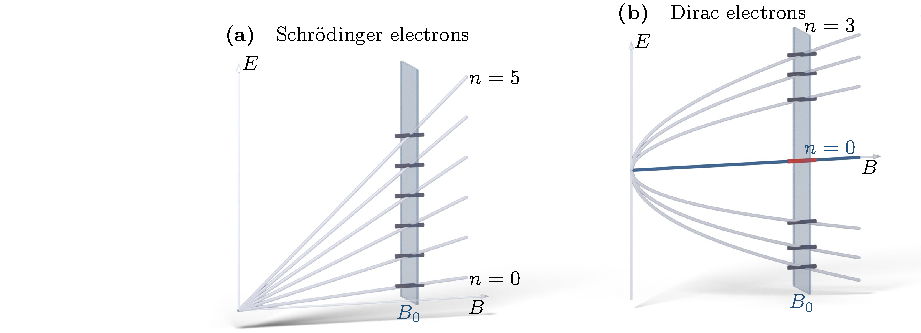
\includegraphics{figures/pdf/s04f04_ladders.pdf}
\end{aqmfigure}


\begin{notebookbox}{\texttt{session4.ipynb}, ``The dispersion of the square lattice'' (Reminder), ``Bands in the conventional quantum Hall state'' (Reminder), ``Landau levels of conventional electrons'' (Core), ``Magnetic field dependence of Landau levels'' (Core), and ``Imaging the magnetic field dependence in the Landau levels'' (Core), together with ``The dispersion of the honeycomb lattice'' (Reminder), ``Bands in the Dirac quantum Hall state'' (Reminder), ``Landau levels of the Dirac equation'' (Core), ``Magnetic field dependence of Dirac Landau levels'' (Core), and ``Imaging the magnetic field dependence in the Dirac Landau levels'' (Core)}
Build a square-lattice ribbon (parabolic band bottom) and a honeycomb-lattice armchair ribbon
(Dirac cone) with the Peierls substitution (4.4) switched on, and confirm both spectra directly:
equally-spaced flat Landau levels growing linearly in $B$ for the square lattice, reproducing
(4.6), against unequally-spaced levels growing as $\sqrt{B}$ for the honeycomb lattice,
reproducing (4.7). The ``imaging'' sections let you track individual level energies as an explicit
function of field strength, which is the most direct numerical check of the linear-versus-square-root
scaling derived above.
\end{notebookbox}

\section{Numerical confirmation: Landau levels and edge states on the lattice}

It is worth being explicit about how the continuum results of Sections 4.9 and 4.10 connect to
tight-binding lattices, since this is where the edge states of Section 4.5 first become visible
alongside the bulk Landau levels in a single calculation. Take a finite-width ribbon of a square
lattice (whose band bottom is parabolic, hence a stand-in for the Schrödinger 2DEG), add a uniform
orbital field through the Peierls substitution (4.4), and set the chemical potential near the
bottom of the band, so the lattice model is effectively describing a dilute, nearly-free electron
gas. The resulting band structure shows exactly what the continuum calculation predicted: a set of
flat bulk bands (the Landau levels) sitting alongside dispersive edge bands, one branch localized
at each edge of the ribbon and propagating in opposite directions, precisely the chiral pair
described in Section 4.5. Repeating the same construction on a honeycomb-lattice armchair ribbon,
whose low-energy physics is a genuine Dirac equation at the $K$ and $K'$ points, reproduces the
$\sqrt{B}$ Landau levels of Section 4.10 together with their own chiral edge states. Both ribbon
band structures (width-30 examples in the slides) are genuinely slide-only figures in the sense
that the transcript only describes them qualitatively; the plots themselves carry the visual
evidence, and building the equivalent ribbons yourself is exactly what the notebook callout above
asks you to do.

\section{Ladder operators and the many-body Landau Hamiltonian}

Sections 4.9 and 4.10 both found harmonic-oscillator structure by working in a specific gauge. We
can make that structure manifest in a gauge-independent way by defining ladder operators directly
from the canonical momentum,

\begin{equation*}
a = \frac{\ell_B}{\sqrt{2}\hbar}(\pi_x + i\pi_y), \qquad a^\dagger = \frac{\ell_B}{\sqrt{2}\hbar}(\pi_x-i\pi_y),
\end{equation*}

which, using only $[\pi_x,\pi_y]=i\hbar^2/\ell_B^2$ (a statement purely about the field, not about
any particular gauge), satisfy the canonical bosonic commutation relation $[a,a^\dagger]=1$. In
terms of these operators the \emph{full} quantum Hall Hamiltonian for a Schrödinger electron becomes

\begin{equation}
H = \hbar\omega_c\left(a^\dagger a + \frac{1}{2}\right),
\end{equation}

manifestly a harmonic oscillator, with eigenvalues reproducing (4.6) directly and with no reference
to a gauge at all. This is the cleanest way to see that ``Landau levels behave like a harmonic
oscillator'' is not an artifact of the Landau gauge; it is a structural property of any electron in
a uniform field.

\section{The symmetric gauge and the lowest-Landau-level wavefunctions}

To go from single-particle Landau levels to a genuinely many-body quantum Hall wavefunction, we
switch to the symmetric gauge, $\mathbf{A}=\tfrac{B}{2}(-y,x,0)$, and to the complex coordinate
$z=x+iy$. Writing $\partial_z = \tfrac12(\partial_x-i\partial_y)$ and $\partial_{\bar z} =
\tfrac12(\partial_x+i\partial_y)$, the ladder operator of Section 4.12 becomes, in this gauge,
proportional to $\partial_{\bar z} + z/4\ell_B^2$. The lowest-Landau-level (LLL) condition, $a\psi=0$,
is therefore the first-order differential equation

\begin{equation}
\left(\partial_{\bar z} + \frac{z}{4\ell_B^2}\right)\psi(z,\bar z) = 0
\quad\Longrightarrow\quad
\psi(z,\bar z) = f(z)\, e^{-|z|^2/4\ell_B^2},
\end{equation}

for an \emph{arbitrary holomorphic function} $f(z)$, that is, any function built only from powers of $z$
and never $\bar z$. This is the precise statement behind ``any power $z^m$ times a Gaussian is a
zeroth-Landau-level wavefunction'': holomorphicity is not an extra assumption, it is exactly what
solving the LLL condition in the symmetric gauge forces on us. The single-particle LLL orbitals are
then

\begin{equation}
\psi_m(z) = z^m\, e^{-|z|^2/4\ell_B^2}, \qquad m=0,1,2,\dots,
\end{equation}

each labeled by an angular momentum $m$ (the eigenvalue of $L_z$ in this gauge), all sharing the
same Gaussian envelope but with the polynomial prefactor $z^m$ pushing the orbital's probability
density further from the origin as $m$ grows, since $|\psi_m|^2$ peaks where $\tfrac{d}{d|z|}\big(|z|^{2m}e^{-|z|^2/2\ell_B^2}\big)=0$,
at radius $r_m = \sqrt{2m}\,\ell_B$.

\section{The many-body wavefunction of the filled lowest Landau level}

Now we ask for the many-body ground state in which \emph{every} LLL orbital is occupied, for $N$
electrons. Two requirements pin this state down completely: it must be built entirely from LLL
orbitals (4.10), and it must be antisymmetric under exchange of any two electrons, as fermion
statistics demands. Both requirements are satisfied at once by

\begin{equation}
\Psi_1(z_1,\dots,z_N) = \prod_{i<j}(z_i-z_j)\; \exp\!\left(-\sum_i \frac{|z_i|^2}{4\ell_B^2}\right).
\end{equation}

The Vandermonde product $\prod_{i<j}(z_i-z_j)$ does two jobs simultaneously. First, it is
automatically antisymmetric: exchanging any two coordinates $z_i\leftrightarrow z_j$ flips the sign
of exactly the one factor $(z_i-z_j)$, giving the overall minus sign Pauli's principle demands.
Second, it is precisely the Slater determinant of the single-particle orbitals
$1,z,z^2,\dots,z^{N-1}$, since $\det\!\big(z_i^{\,j-1}\big) = \prod_{i<j}(z_j-z_i)$ is the standard
Vandermonde determinant identity, so (4.11) is nothing but the Slater determinant of all $N$
lowest LLL orbitals, times their common Gaussian envelope (the individual Gaussians simply combine
into the single collective exponential shown). This is the exact many-body ground state of $N$
electrons filling the lowest Landau level completely: the integer quantum Hall state at filling
$\nu=1$.

\section{Angular momentum, enclosed flux, and the uniform electron gas}

Section 4.13 already told us that larger angular momentum $m$ pushes an orbital's peak further from
the origin, to radius $r_m=\sqrt{2m}\,\ell_B$; equivalently, that orbital encloses a larger area,
and therefore a larger amount of magnetic flux. This link between angular momentum and enclosed
flux is what we will use in Section 4.17 to track how much charge a quasiparticle carries. For now,
the important consequence is about (4.11) itself: summing over the full Slater determinant, one
finds a density profile that is essentially uniform (flat) out to a radius set by the highest
occupied angular momentum $m=N-1$, and falls sharply to zero beyond it. The filled lowest Landau
level, in other words, is a genuinely featureless, uniform two-dimensional electron gas, which is
exactly the property we will now ask a \emph{fractionally} filled Landau level to share.
Figure~\ref{fig:s04:droplet} shows both halves of that statement: the individual orbitals as
nested rings of growing radius, and the flat droplet they add up to.

% Session 4 -- lowest-Landau-level orbitals as nested rings, and the uniform
% droplet they add up to at nu=1 and at nu=1/3.
% Placement: sec. "Angular momentum, enclosed flux, and the uniform electron gas".
% Rendered by figures/blender/s04f05_droplet.py, labels in figures/overlays/s04f05_droplet.tex.
\begin{aqmfigure}{fig:s04:droplet}{Angular momentum fixes the radius. (a) The lowest-Landau-level
orbitals (4.10), $|\psi_m|^2\propto r^{2m}e^{-r^2/2\ell_B^2}$, for $m=0,2,4,6,8$, each renormalized
here to the same peak height and cut open over half a turn. They are nested rings, and when $m$
increases the ring moves outward, to $r_m=\sqrt{2m}\,\ell_B$, and encloses more flux. (b) When we
add every orbital from $m=0$ to $m=N-1$ we therefore fill a disc, and the rings overlap in such a
way that the total density is flat inside the disc and falls off sharply at the edge. The filled
lowest Landau level is a uniform electron droplet without structure, with one electron per flux
quantum. The Laughlin state (4.12) at $\nu=1/3$ is the second profile. The same $N$ electrons now
use orbitals up to $m=3(N-1)$, so the radius of the droplet grows by $\sqrt{3}$ and the density
becomes a third, while the droplet stays as uniform as before. The Laughlin construction is built to
keep this uniformity, and the profiles of (b) are schematic.}
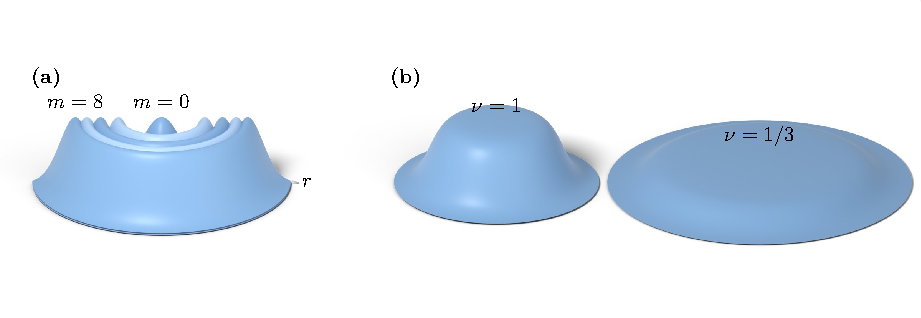
\includegraphics{figures/pdf/s04f05_droplet.pdf}
\end{aqmfigure}


\section{Fractional filling and the Laughlin wavefunction}

Suppose instead we want to occupy only a fraction of the available LLL orbitals, say two out of
every three, but in a way that keeps the electron gas uniform rather than simply leaving isolated
orbitals empty (which would create an obviously non-uniform, ``lumpy'' density, since each empty
orbital sits at its own fixed radius). What we are looking for is a many-body wavefunction that:
still lives entirely in the LLL, so it is built only from the coordinates $z_i$ and never $\bar
z_i$; is still antisymmetric, since the particles are still electrons; and, heuristically, keeps the
electrons as far apart from one another as possible, since that is what minimizing a repulsive
Coulomb interaction energy would favor.

The construction that achieves all three requirements at once is remarkably simple: take the
filled-LLL wavefunction (4.11) and raise the Vandermonde factor to a power,

\begin{equation}
\Psi_m(z_1,\dots,z_N) = \prod_{i<j}(z_i-z_j)^m\; \exp\!\left(-\sum_i \frac{|z_i|^2}{4\ell_B^2}\right),
\end{equation}

the \textbf{Laughlin wavefunction}. The exponent $m$ must be an odd integer: an even power would make
the wavefunction \emph{symmetric} rather than antisymmetric under exchange, which fermions cannot allow.
Raising the exponent directly increases the ``avoidance'' between electrons (the wavefunction now
vanishes to $m$-th order, not just linearly, whenever two electrons coincide), which is exactly the
correlation effect we were after. Working out the resulting electron density gives filling factor

\begin{equation}
\nu = \frac{1}{m},
\end{equation}

which one can see directly by counting: the maximum power of any single coordinate appearing in the
fully expanded polynomial (4.12) is $m(N-1)$, so the wavefunction uses angular-momentum orbitals up
to $m(N-1)$, meaning $N$ electrons are spread over $\approx m(N-1)+1 \approx mN$ available LLL
orbitals, a filling fraction of $N/(mN)=1/m$, matching (4.13). It is worth pausing on how
remarkable this construction is: starting from nothing but the single-particle LLL orbitals,
Pauli's exclusion principle, and a heuristic correlation argument, we land on the exact ground
state of a strongly interacting many-body problem, and it is going to hand us fractional charge in
the very next section.

\section{Quasiholes and quasielectrons}

\emph{From this point through the end of Section 4.18, the material has no counterpart in
\texttt{session4.ipynb}. The notebook's coverage of this session stops at the integer quantum Hall state,
its Landau levels, and its edge and Chern-insulator physics (Sections 4.10, 4.11, and 4.19 below);
the Laughlin wavefunction, quasiholes and quasielectrons, and the Berry-phase argument for
fractional charge and anyonic statistics are transcript-and-slide material with no numerical
exercise built around them.}

Excitations above the Laughlin ground state (4.12) turn out to have an equally simple construction
in these coordinates. A \textbf{quasihole} at the origin is obtained by multiplying the wavefunction by
an extra overall factor of $z_i$ for every electron; a quasihole at an arbitrary location $w$ is
obtained instead by inserting a factor $(z_i-w)$ for each electron,

\begin{equation}
\Psi_{\text{qh}}(w) = \prod_i (z_i-w) \; \Psi_m(z_1,\dots,z_N).
\end{equation}

Multiplying by this extra factor raises the effective power associated with every orbital by one,
which, by the angular-momentum-versus-radius relation of Section 4.15, pushes charge density
outward, away from $w$, leaving a depleted region there: a quasihole. Repeating this construction
$m$ times, at $m$ different locations, removes exactly one full electron's worth of charge overall,
consistent with each individual quasihole carrying only a fraction $1/m$ of an electron charge (we
will confirm this fraction directly via the Berry phase in Section 4.18). A \textbf{quasielectron} is, in
this same language, the inverse operation: instead of raising the power (multiplying by
$z_i-w$), we lower it, implemented by a derivative with respect to $z_i-w$ rather than a
multiplication; this pulls charge inward instead of pushing it outward, giving an excitation of
opposite (negative) fractional charge.

\section{Berry phase, fractional charge, and anyonic statistics}

We now use the Berry phase, the same object session 3 built the Chern number from, to show
directly that the quasihole excitation of Section 4.17 really does carry a fraction of an electron
charge, and that a pair of them obey neither fermionic nor bosonic exchange statistics.

\textbf{Fractional charge.} Take the single-quasihole wavefunction (4.14) and adiabatically move $w$
around a closed loop, parameterizing $w=|w|e^{i\theta}$ and computing the resulting Berry phase as
$\theta$ runs from $0$ to $2\pi$. The result comes out as an Aharonov-Bohm phase, proportional to
the flux enclosed by the loop, but carrying an extra prefactor of $1/m$ relative to what an ordinary
charge-$e$ particle would pick up around the same loop. Since the Aharonov-Bohm phase for a particle
of charge $q$ around enclosed flux $\Phi$ is $2\pi q\Phi/\Phi_0$ (with $\Phi_0$ the flux quantum),
the extra $1/m$ we find is a direct, unambiguous statement about the \emph{charge} of the excitation:

\begin{equation}
q_{\text{qh}} = \frac{e}{m}.
\end{equation}

The electron is no longer the fundamental unit of charge for these excitations; a genuine fraction
of it is.

\textbf{Anyonic statistics.} Now take a wavefunction with \emph{two} quasiholes, one fixed at the origin and
one at $w$, and move the second one in a loop around the first, again parameterizing
$w=|w|e^{i\theta}$. The resulting Berry phase splits into two pieces: the same Aharonov-Bohm
contribution as before (charge times enclosed flux), plus an additional \textbf{statistical phase}
picked up purely from winding one quasiparticle around the other,

\begin{equation}
\theta_{\text{stat}} = \frac{2\pi}{m}.
\end{equation}

One bookkeeping point matters when comparing this to the familiar cases: taking one quasiparticle
all the way around another is \emph{two} successive exchanges, so the exchange phase is half of
(4.16), namely $\pi/m$. For ordinary fermions, exchanging two particles gives a phase of $\pi$; for
bosons, a phase of $0$. The exchange phase $\pi/m$ is neither, and it interpolates between the two
familiar cases as $m$ grows (see figure~\ref{fig:s04:quasihole}): these quasiparticles are \textbf{anyons}, excitations whose exchange
statistics interpolate continuously between the fermionic and bosonic cases, labeled by the same
integer $m$ that set the filling fraction. We started from a many-body wavefunction built entirely
out of ordinary electrons, genuine fermions, and out of that wavefunction's own correlations we have
produced excitations that are neither fermions nor bosons: this is the simplest example of
fractionalization in a quantum many-body system that we will meet in this course.

% Session 4 -- the Laughlin quasihole: a depletion of fractional charge, and the
% Berry phase that measures both its charge and its exchange statistics.
% Placement: sec. "Berry phase, fractional charge, and anyonic statistics",
% after equation (4.16).
% Rendered by figures/blender/s04f06_quasihole.py, labels in figures/overlays/s04f06_quasihole.tex.
\begin{aqmfigure}{fig:s04:quasihole}{Fractional charge and fractional statistics, both obtained from
a Berry phase. (a) When we multiply the Laughlin state by $\prod_i(z_i-w)$, equation (4.14), the
angular momentum of every electron about $w$ increases by one, which by figure~\ref{fig:s04:droplet}
moves charge radially outward and leaves a region with less charge behind, the dimple. If we do this
$m$ times we remove exactly the charge of one electron, so one quasihole has the charge of an
electron divided by $m$, which is $q=e/m$. (b) When we move one quasihole once around another, along
the loop, and follow the Berry phase, it separates into two parts. The first is an Aharonov-Bohm
part, proportional to the enclosed flux, and its prefactor is what fixes $q=e/m$ in (4.15). The
second is a remaining part $2\pi/m$, which depends only on the fact that one quasiparticle went
around the other. A full loop is two exchanges, so the exchange phase itself is $\pi/m$, drawn at
the bottom for $m=3$. For every odd $m>1$ it is strictly between the bosonic $0$ and the fermionic
$\pi$, and this is what makes these excitations anyons.}
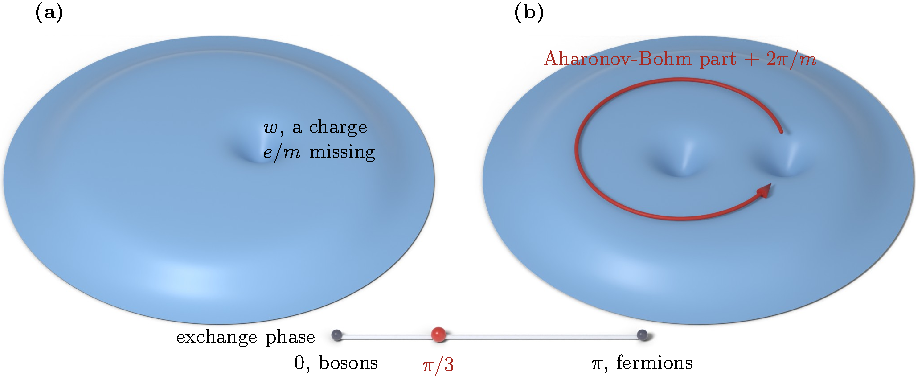
\includegraphics{figures/pdf/s04f06_quasihole.pdf}
\end{aqmfigure}


\section{The quantum Hall effect without Landau levels: the Haldane model, revisited}

This closing section is a deliberate callback, not new material: session 3 already built the
Haldane model, as its own worked example of a Chern insulator obtained by gapping a Dirac cone
without any external field. We revisit it here specifically because it closes the loop this
session opened: everything above required an actual magnetic field to produce Landau levels, so it
is worth confirming explicitly that the quantized Hall conductance itself never actually required
one.

As a quick reminder of the construction: start from the honeycomb lattice with first-neighbor
hopping only (an ungapped Dirac cone at $K$ and $K'$), and add a second-neighbor hopping that is
purely imaginary, which breaks time-reversal symmetry. In the Bloch Hamiltonian this term appears
as a valley-dependent mass, with opposite sign at $K$ and $K'$ for an ordinary staggered on-site
potential, but with the \emph{same} sign at both valleys for the Haldane (imaginary second-neighbor)
term. Equal-sign masses at both valleys give equal-sign Berry curvature at both valleys too, so the
two valley contributions add rather than cancel when integrated over the Brillouin zone, leaving a
net, nonzero Chern number, an insulating bulk gap, and a chiral edge state, all with $B=0$
throughout.

What is genuinely new in today's version of this story is the explicit \textbf{adiabatic connection}
between the Haldane model and the ordinary field-driven quantum Hall state of this session. Start
in the Haldane model (imaginary second-neighbor hopping, no field); switch on a real magnetic field
while keeping the Haldane coupling, and Landau levels develop out of the previously dispersive
bands; then switch the Haldane coupling back off, leaving the system in the ordinary quantum Hall
state built from Landau levels alone. At every step of this path the bulk gap stays open and the
chiral edge state never disappears. Since the two end points can be connected without ever closing
the gap, the Haldane-model Chern insulator and the Landau-level quantum Hall state are
\emph{topologically equivalent}: the very same phase of matter, reached by two completely different
physical routes, one that needs a magnetic field and one that does not.

\begin{notebookbox}{\texttt{session4.ipynb}, ``Topological equivalence between the Quantum Hall state and a Chern insulator'' (Challenge), and ``Topological domains in the quantum Hall state'' (Challenge)}
Build the Haldane model, turn a magnetic field on and off numerically alongside the Haldane
coupling, and track the bulk gap and Chern number through the adiabatic path described above.
The ``topological domains'' exercise lets you probe spatial regions where the two couplings
compete directly, a hands-on version of the equivalence argument just given.
\end{notebookbox}

\section{Real materials realizing Chern and fractional Chern physics}

\emph{This survey, like Section 4.17-4.18, is transcript-and-slide content with no notebook
counterpart; there is no numerical exercise in \texttt{session4.ipynb} built around any of the specific
compounds below.}

The zero-field Chern insulator is not just a theoretical curiosity. Chromium-doped
$(\text{Bi,Sb})_2\text{Te}_3$, a magnetically doped topological insulator, breaks time-reversal
symmetry through genuine magnetism and realizes an integer quantized Hall conductance with no
applied field. Twisted graphene bilayers aligned with a boron nitride substrate realize the same
physics through a different mechanism, orbital currents rather than magnetic moments. On the
fractional side, twisted two-dimensional materials can host topological flat bands whose
mathematical structure mimics an artificial, pseudo-magnetic field tied to elastic lattice
reconstruction rather than any real field; twisted bilayers of molybdenum ditelluride
(MoTe$_2$) are a recent, striking example, showing genuine fractional quantum Hall physics at zero
magnetic field.

\section{Closing summary}

\begin{itemize}
\item The Hall conductivity is a topological invariant, the Chern number of the occupied bands,
  exactly as derived (more fully) in session 3; equation (4.1) is the same result confirmed once
  more here rather than re-derived from scratch.
\item A magnetic field turns a two-dimensional electron gas into a set of flat Landau levels, each
  carrying Chern number one, so the Hall conductivity is quantized to $N e^2/h$ for $N$ filled
  Landau levels, equation (4.2).
\item An insulating bulk still conducts because a nonzero Chern number forces chiral, backscattering-free
  edge states at the sample boundary (Section 4.5), directly visible in ribbon band structures.
\item Landau levels arise from minimal coupling (4.3) or, on a lattice, the Peierls substitution (4.4);
  Schrödinger electrons give equally spaced levels $E_n=\hbar\omega_c(n+\tfrac12)$, equation (4.6),
  while Dirac electrons give $E_n\propto\sqrt{nB}$, equation (4.7), explaining graphene's much
  higher quantum Hall temperature scale.
\item In the symmetric gauge, lowest-Landau-level wavefunctions are holomorphic, $\psi_m(z)\propto
  z^m e^{-|z|^2/4\ell_B^2}$, equation (4.10); the filled-LLL many-body state is the Vandermonde
  determinant times a collective Gaussian, equation (4.11).
\item Raising the Vandermonde factor to an odd power $m$ gives the Laughlin wavefunction, equation
  (4.12), with filling factor $\nu=1/m$, equation (4.13); its quasihole excitations, equation
  (4.14), carry fractional charge $e/m$, equation (4.15), and obey anyonic statistics, picking up
  $2\pi/m$ on a full braid, equation (4.16), that is an exchange phase $\pi/m$ strictly between the
  bosonic $0$ and the fermionic $\pi$: the simplest instance of fractionalization we will meet.
\item The Haldane model shows the quantized Hall conductance never strictly required a magnetic field
  at all, and is adiabatically, topologically equivalent to the field-driven quantum Hall state, a
  callback to session 3 rather than new machinery.
\end{itemize}

Today's order was driven entirely by a magnetic field, an external, symmetry-breaking knob we
simply turned on by hand. Next session we meet a completely different route to order: attractive
interactions between electrons themselves, driving the system to superconduct without any external
field at all, and we will see that the very same trivial-versus-chiral topological classification
built here and in session 3 comes right back to sort superconducting order parameters into
conventional and topological classes. It is also worth holding on to the flavor of fractionalization
we just built, since we will meet a second, quite different-looking instance of it very soon: here,
correlations inside a partially filled topological flat band split the electron's charge and turned
its exchange statistics anyonic; next time, pairing correlations in a superconductor will split the
electron into Majorana halves instead. Same underlying idea, a correlated topological state hosting
excitations that are not the electron itself, reached by two genuinely different mechanisms.
